% ----------------------------------------------------------------
% Article Class (This is a LaTeX2e document)  ********************
% ----------------------------------------------------------------
\documentclass{article}
\usepackage[english]{babel}
\usepackage{styfiles/proof, styfiles/code, amsmath,amsthm}
\usepackage{amssymb}  % for "\leadsto"
\usepackage{bbold}%for typeface: mathbb
\usepackage{graphicx} %to insert pic from file
\usepackage{hyperref}
% THEOREMS -------------------------------------------------------
\newtheorem{thm}{Theorem}[section]
\newtheorem{cor}[thm]{Corollary}
\newtheorem{lem}[thm]{Lemma}
\newtheorem{prop}[thm]{Proposition}
\theoremstyle{definition}
\newtheorem{defn}[thm]{Definition}
\theoremstyle{remark}
\newtheorem{rem}[thm]{Remark}
\numberwithin{equation}{section}

% ----------------------------------------------------------------
\begin{document}

\newcommand{\env}[1]{[\![#1]\!]\kappa}
\newcommand{\round}[1]{(\!|#1|\!)}

\title{Garbage Collection}%
\author{Di Zhao}%
%\address{address}%
%\thanks{}%\sqrt{}
\date{\small{\texttt{zhaodi01@mail.ustc.edu.cn}}}%
% ----------------------------------------------------------------

\maketitle
% ----------------------------------------------------------------

This is the fourth assignment of Advanced Topics in Software
Technologies. In the previous assignment, we implemented the allocation
and code generation procedure, so that your Monkey compiler is able to
generate C code that can be compiled by some C compiler and then executed.
 However, the memory management strategy we
were using simply allocates memory spaces when needed and never reuse them.
Though logically this would not affect the result of a program, it will
require a lot of memory spaces and in this way a program with complicate
computation may not be able to run on a concrete machine.

To solve this problem, we need to extend the runtime system with
a garbage collection algorithm. The garbage collection algorithm will be
responsible to manage memory space allocations and the reuse of the memory
cells holding values that will never be used again (no longer reachable).
It is your task in this lab to implement the interface between the
compiler and the runtime system.

\section{Memory Layout}

Firstly let us consider the memory layout of structured values.

 The garbage
collector needs to scan over the heap to discard the unreachable values
 and thus make room for further allocations. So it needs to distinguish between
 nun-structured values (such as integers or constant strings) and structured values
 (tuples and tagged values), for the reason that the latter may contain pointers
 to other structured values and thus call for recursive scanning.

Moreover, the garbage collector needs the information to decide how to scan over
a specific tuple or tagged value. Especially, it needs to know when it is done with
a tuple or tagged value. For this reason, we need to store the number of components
in a tuple structure, and distinguish between tuples and tagged values.

To serve the above needs, we can design the memory layout as Figure 1 and Figure 2.
(You may come up with your own designs, as long as they work properly.)

\begin{figure}
  \centering
  % Requires \usepackage{graphicx}
  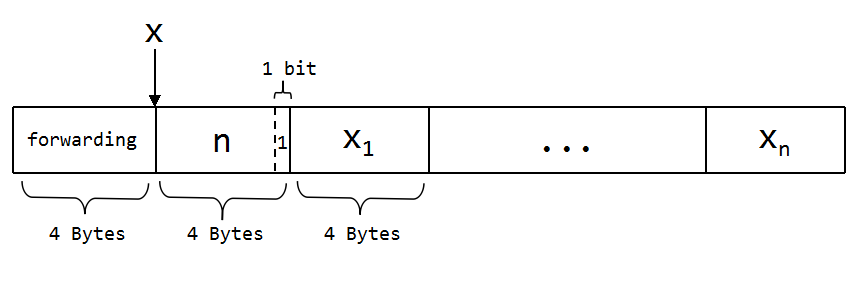
\includegraphics[width=0.98\textwidth]{tuple_gc.png}\\
  \caption{memory layout for tuple: $x=(x_1,\ ...,\ x_n)$}\label{fig:digit}
\end{figure}

\begin{figure}
  \centering
  % Requires \usepackage{graphicx}
  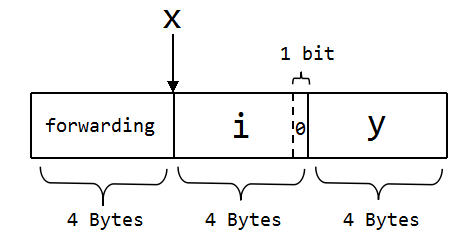
\includegraphics[width=0.55\textwidth]{tag_gc.png}\\
  \caption{memory layout for tagged value: $x=\textsf{in}_i\ y$}\label{fig:digit}
\end{figure}

\begin{figure}
  \centering
  % Requires \usepackage{graphicx}
  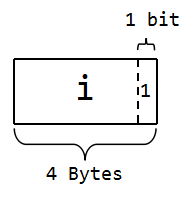
\includegraphics[width=0.22\textwidth]{int_gc.png}\\
  \caption{memory layout for integer $i$}\label{fig:digit}
\end{figure}

Comparing with the strategy we used in the previous lab, the key changes are:
\begin{itemize}
  \item To scan the heap, we need to distinguish between integers, string pointers and
  pointers to tuples and tagged values (because we won't scan along strings and integers).
   The situation is simple for strings: they are
  in the static area, outside the heap that is managed by garbage collector.
  As for boolean values, \texttt{true} is represented by 1 while \texttt{false}
   is represented by 0,
  which means none of the boolean values can be identified as a pointer.

  However, an integer may has the same value with a pointer to the heap.
  To solve this problem,
  here we use the first 31 bits to store a integer's value, and mark the last bit with "1"
  (shown in Figure 3). In contrast, a memory address would never be an odd value,
   its last bit will always be "0". You may have noticed that this method shrinks
   of the domain of integer values.
  \item Figure 1 and Figure 2 reveal how to distinguish between tagged values and tuples.
  (Here we are talking about structures stored in heap, rather than pointers to these
  structures.) The idea is: for a tuple $x=(x_1,\ ...,\ x_n)$, set the last bit of $x[0]$
  to "1"; and for a tagged value $z=\textsf{in}_i\ y$, set the last bit of $z[0]$
  to "0". As a result, there are 31 bits left for a tuple to store its length and a
  tagged value to store its tag.
  \item As you will see in the next section, we use the copying garbage collection
  algorism, thus a "forwarding" field is required to suggest whether a structure is
  copied already and hold the pointer to the new copy. In Figure 1 and Figure 2,
  we place the "forwarding" field ahead of the structures. In other word, $x[-1]$ stores
  the forwarding pointer for a tuple or a tagged value $x$.
\end{itemize}

To be mentioned, to support garbage collection, the heap is divided to two separate zones:
 "to" and "from". The dynamic allocated structures are placed in the "from" zone. \\


\section{Garbage Collection}

The garbage collection algorism is mostly the same with the Tiger compiler (course:
\textit{Compiler}). You can refer to
\href{http://staff.ustc.edu.cn/~bjhua/courses/compiler/2014/labs/lab4/index.html}
{lab 4 of Compiler} for the details. If you are unfamiliar with this,
you should read Tiger book chapter 13.3 first.
 Make sure you understand Cheney's algorithm thoroughly before continuing.

Unlike the Tiger compiler, here garbage collection is performed each time
  before a function call. In this way, we can safely assume that there's only
  one active value when the garbage collector runs, i.e. the argument to be
  passed. In \texttt{runtime.c}, the external variable \texttt{\_arg} represented
  this argument. The whole point for this change is to simplify the
  implementation. Otherwise we would need a memory map for the locals of the
  active function, and scan the stack base on this map when performing garbage
  collection.


\section{Code Generation}

To support garbage collection, we need to make some changes in the code
generation procedure, so that the generated code will cooperate well
with our runtime system. In this section, it is your task to implement the
new code generation procedure. Listed below are the new characteristics:
\begin{itemize}
  \item The runtime stack is eliminated. After the CPS conversion, function
  will never return. Consequently, it will be a waste of spaces to generate
  C code directly, for the stack frames will be continually accumulated
  yet never be popped off, until the entire program terminates.

  $\ \ $The problem can be solved by two steps:
  \begin{enumerate}
    \item The \texttt{main} function continuously calls one global function pointer
    (denoted as "\texttt{\_f}") in a loop. Use another global value (denoted as
    "\texttt{\_arg}") to hold the argument.
    \item In the generated functions, instead of calling another function directly,
    assign the callee to the global function pointer \texttt{\_f}, assign its
    argument to the global argument value \texttt{\_arg}, and then simply return.
    As a result, the callee will be called by the \texttt{main} function immediately.
  \end{enumerate}
    Now the stack will have at most 2 frames: one for the \texttt{main}
    function, another for the current function to be executed.
  \item Now that the memory layout for integers has changed, you have to make some changes
  in code generation to reflect this:
  \begin{enumerate}
    \item The output of constant integer values: perform a logical left shift and set
    the last bit to 1.
    \item The primary operations on integers: \textit{add}, \emph{sub} and \emph{times}
    operations are now output as function calls to \texttt{ml\_add}, \texttt{ml\_sub} and
     \texttt{ml\_times}.
  \end{enumerate}
  \item As the garbage collection procedure take place before a function call (rather than
  in an allocation procedure), we need to decide whether the current heap has enough spaces
  for the function to run. Consequently, we need to obtain the information of how many
  memory spaces a function needs. Luckily as the ML language doesn't contain
  any loop statements, we can obtain the upper bound of this number by simply adding up the
  sizes of tuples and tagged values in a function.

  $\ \ $Consider by yourself, how to calculate this size value for each function, and how
  to obtain this value
  (in the output code) to perform garbage collection in \texttt{main}  before
   calling a function.
\end{itemize}

\noindent{
\fbox{%
\parbox{\textwidth}{%
Functions in \texttt{gc.sml} to output the Machine
 syntax tree as C code (accordance with the garbage collector in
  \texttt{runtime.c}).
 \begin{itemize}
   \item Finish \texttt{dumpFunc} to print a function. Consider:
   \begin{itemize}
     \item how to calculate the number of Bytes needed to run the function
   (hint: you can use a reference to hold the value and add to this value
   in \texttt{dumpValue});
     \item how to output these functions' sizes in the C code,
     so that before each call of \texttt{\_f(\_arg)} in \texttt{main}, you can call
     \texttt{Gc\_retrieve(n)} with the proper \texttt{n}.
   \end{itemize}
    \item Finish \texttt{dumpValue} to print a term of Machine.Binding.v. Consider:
    \begin{itemize}
      \item how to output an constant integer;
      \item basic operations on integers should be printed as invoking of
      the corresponding library function in the runtime system;
      \item how many Bytes are needed for a tuple or a tagged value.
    \end{itemize}
   \item Finish \texttt{dumpExp} to print a term of Machine.Block.exp.
   \begin{itemize}
     \item For a function call \texttt{fname(x)}, your output should assign \texttt{\_f}
     with \texttt{fname} and assign \texttt{\_arg} with \texttt{x}, and then simply returns.
     \item For if0 expression, pay attention to the judgment of the condition as the
     representation of integers has changed.
     \item For a case expression, pay attention to the switch cases, according to the
     memory map of tagged value (Figure 2).
   \end{itemize}
   \item Finish \texttt{dumpmain} to print the main function. You should:
   \begin{itemize}
     \item initialize the global variables "\texttt{\_f}" and "\texttt{\_arg}" with
     "\texttt{ml\_main}" and 0 (why?) respectively;
     \item initialize the heap;
     \item call \texttt{\_f(\_arg)} in a loop;
     \item before each call of \texttt{\_f(\_arg)}, call \texttt{Gc\_retrieve(n)}
     to perform garbage collection if needed. Here \texttt{n} is the spaces (number
     of Bytes) needed to run \texttt{\_f}.
   \end{itemize}
 \end{itemize}
}
}
}

\noindent{
Updates:
\begin{description}
  \item[15-7-6] Modified \texttt{gc.sml} to support multiple cases.

  \textcolor[rgb]{1.00,0.00,0.00}{Note:} the generated executive file
  takes an argument as the number of bytes of the initial heap size (2000 by default).
  
   \item[15-9-5:]
  Added boolean values and corresponding operations. Changed \texttt{if0}
  expression into \texttt{if} expression.
\end{description}
}


\end{document}
